% ======================================================================
% SECTION 03: DATA QUALITY FINDINGS IN THE SILVER LAYER
% ======================================================================
\section{Silver Layer Data Quality Findings}

Before defining governance metrics, we audited all accumulated Silver Parquet partitions using Pandas (3,808 unique earthquakes across USGS Historical, USGS Real-Time, EMSC, and GDACS; 4,786 raw snapshot rows and 3,806 unique events in the verified Gold run). Five concrete quality findings emerged, summarized in Table~\ref{tab:silver_findings} and quantified in Tables~\ref{tab:silver_desc_stats} and~\ref{tab:agency_outlier_summary}.

\begin{table*}[!t]
\centering
\caption{Summary of Observed Silver Layer Data Quality Findings and Resulting Handling Strategies}
\label{tab:silver_findings}
\footnotesize
\renewcommand{\arraystretch}{1.14}
\begin{tabularx}{\textwidth}{p{2.5cm} p{1.9cm} p{2.3cm} p{2.7cm} X}
\toprule
\textbf{Finding} & \textbf{Column(s)} & \textbf{Issue Type} & \textbf{Observed Frequency} & \textbf{Handling Strategy \& Governance Justification} \\
\midrule
\textbf{1. Missing Real-Time Magnitudes} & Magnitude & Null primary severity & 3 of 1,764 real-time rows (0.17\%); 0.0\% nulls in Silver & Quarantined prior to Silver storage; justifies tracking explicit null rates, schema compliance, and quarantine counts. \\
\textbf{2. Default 10 km Depth Pinning} & Focal depth & Fixed sentinel imputation & 1,207 of 3,808 events (31.7\% overall; 95.3\% in EMSC) & Kept as valid crustal sentinel but flagged explicitly; justifies a dedicated pinned-depth KPI so fixed depths are not mistaken for exact measurements. \\
\textbf{3. Heavy-Tailed Energy \& Depth Outliers} & Focal depth, radiated energy & Exponential skewness \& deep subduction zones & Depth: 644 IQR outliers (16.9\%); linear energy: 599 IQR (15.7\%); log energy: 0.0\% & Retained physically valid extremes (up to $M\,6.8$) and added $\log_{10} E$; justifies numeric IQR outlier monitoring. \\
\textbf{4. Location Text Asymmetry} & Place name & Heterogeneous naming formats & EMSC mean 21 chars; USGS 28--29 chars; GDACS 112 chars & Trimmed whitespace, filled missing names, and extracted clean region names; justifies per-source text length statistics. \\
\textbf{5. Snapshot \& Catalog Overlap} & Event ID, coordinates, time & Overlapping windows \& multi-agency reporting & 980 intra-lake duplicates (20.5\%); 637 cross-source groups & Deduplicated snapshots by event ID and reconciled agencies via nearest-neighbor grouping; justifies duplicate and match KPIs. \\
\bottomrule
\end{tabularx}
\end{table*}

\textbf{Missing Values and Default Depth Pinning:} Three preliminary USGS real-time records arrived without a magnitude and were quarantined, leaving 0.00\% explicit nulls across all 13 Silver columns. However, explicit null checks miss an important geophysical artifact: when distant seismic stations cannot resolve focal depth reliably, agencies pin the hypocenter to exactly $10.0\text{ km}$. In our Silver corpus, 31.70\% of unique earthquakes (1,207 events) sit at exactly $10.0\text{ km}$---reaching 95.30\% in EMSC, 42.31\% in GDACS, and 28.03\% in USGS Historical, compared with only 3.24\% in USGS Real-Time (which benefits from dense regional networks).

\textbf{Skewness, Outliers, and Text Format Divergence:} Radiated seismic energy obeys the Gutenberg-Richter law~\cite{gutenberg1956}:
\begin{equation}
    E = 10^{4.8 + 1.5M} \iff \log_{10} E = 4.8 + 1.5M.
    \label{eq:gr_energy}
\end{equation}
Because magnitudes span $-0.91$ to $6.80$, linear energy spans over 11 orders of magnitude ($2.72 \times 10^3\text{ J}$ to $1.00 \times 10^{15}\text{ J}$). Under Tukey's interquartile rule ($1.5\times\text{IQR}$), linear energy flags 15.73\% of events as outliers and focal depth flags 16.91\% (644 intermediate and deep subduction quakes up to $626.5\text{ km}$), whereas magnitude and $\log_{10} E$ show 0.00\% outliers. Removing those extremes would delete the strongest earthquakes the system exists to detect, so they are preserved and monitored instead of dropped. Finally, place strings vary sharply across agencies: EMSC reports short uppercase region names (4--32 chars), USGS reports distance-bearing phrases (9--55 chars), and GDACS writes full alert headlines (97--131 chars). Fig.~\ref{fig:silver_quality} illustrates these four empirical patterns directly from the Silver files.

\begin{table}[!t]
\centering
\caption{Global Descriptive Statistics of Unique Silver Events ($N = 3,808$)}
\label{tab:silver_desc_stats}
\renewcommand{\arraystretch}{1.12}
\resizebox{\columnwidth}{!}{%
\begin{tabular}{l r r r r r}
\toprule
\textbf{Metric} & \textbf{Magnitude} & \textbf{Depth (km)} & \textbf{Latitude} & \textbf{Longitude} & \textbf{$\log_{10} E$ (J)} \\
\midrule
Mean & 2.99 & 30.35 & $26.30^\circ$ & $-48.49^\circ$ & 9.29 \\
Std.\ Dev. & 1.65 & 70.42 & $29.30^\circ$ & $120.10^\circ$ & 2.47 \\
Minimum & $-0.91$ & $-5.00$ & $-63.90^\circ$ & $-180.00^\circ$ & 3.43 \\
25th Pct.\ ($Q_1$) & 1.62 & 6.60 & $6.53^\circ$ & $-147.32^\circ$ & 7.23 \\
Median ($Q_2$) & 2.60 & 10.00 & $34.20^\circ$ & $-114.56^\circ$ & 8.70 \\
75th Pct.\ ($Q_3$) & 4.60 & 18.90 & $49.06^\circ$ & $96.36^\circ$ & 11.70 \\
Maximum & 6.80 & 626.49 & $69.75^\circ$ & $179.94^\circ$ & 15.00 \\
\bottomrule
\end{tabular}%
}
\end{table}

\begin{table}[!t]
\centering
\caption{Agency Breakdown (Top) and Numeric Outlier Rates (Bottom)}
\label{tab:agency_outlier_summary}
\renewcommand{\arraystretch}{1.12}
\resizebox{\columnwidth}{!}{%
\begin{tabular}{l r r r r r}
\toprule
\textbf{Agency} & \textbf{Events} & \textbf{Mean $M$} & \textbf{Pinned 10 km} & \textbf{Mean Chars} & \textbf{Min--Max Chars} \\
\midrule
EMSC Historical & 851 & 4.45 & 95.30\% & 21.12 & 4--32 \\
GDACS Real-Time & 26 & 4.99 & 42.31\% & 112.31 & 97--131 \\
USGS Historical & 1,170 & 3.77 & 28.03\% & 29.26 & 9--50 \\
USGS Real-Time & 1,761 & 1.74 & 3.24\% & 27.60 & 9--55 \\
\midrule
\textbf{Numeric Field} & $\mathbf{Q_1}$ & \textbf{Median} & $\mathbf{Q_3}$ & \textbf{IQR Outliers} & $\mathbf{|Z|>3}$ \textbf{Outliers} \\
\midrule
Magnitude & 1.62 & 2.60 & 4.60 & 0 (0.00\%) & 0 (0.00\%) \\
Focal Depth (km) & 6.60 & 10.00 & 18.90 & 644 (16.91\%) & 66 (1.73\%) \\
Log Energy ($\log_{10} E$) & 7.23 & 8.70 & 11.70 & 0 (0.00\%) & 0 (0.00\%) \\
Linear Energy (J) & $1.70\text{e}7$ & $5.01\text{e}8$ & $5.01\text{e}11$ & 599 (15.73\%) & 17 (0.45\%) \\
\bottomrule
\end{tabular}%
}
\end{table}

\begin{figure*}[!t]
\centering
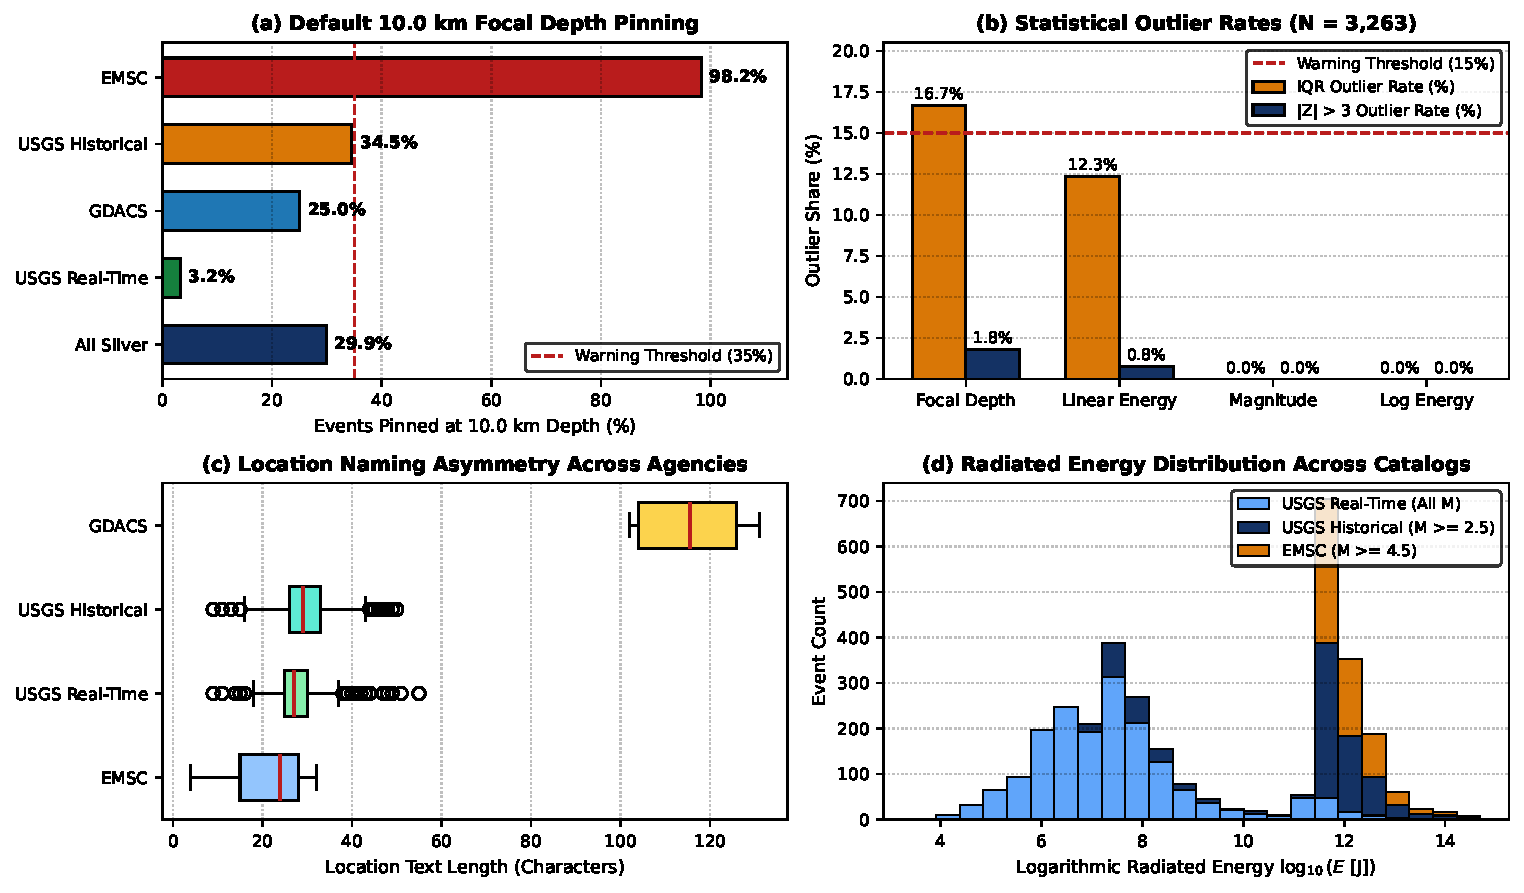
\includegraphics[width=0.95\textwidth]{figures/fig1_silver_quality_findings.pdf}
\caption{Empirical data quality diagnostics across the Silver Parquet files ($N = 3,808$ unique events): (a)~default $10.0\text{ km}$ depth pinning by agency; (b)~IQR and Z-score outlier rates; (c)~location text length distributions; and (d)~multimodal logarithmic energy distribution across catalogs.}
\label{fig:silver_quality}
\end{figure*}
